% Source: graduate-coursework/Research/How_to_write/00_Contrastive_Synthesis.tex
% Description: \textbf{Current-Traditional Rhetoric.

\documentclass[border=4pt]{standalone}
\usepackage{newtxtext,newtxmath}
\usepackage{tikz}
\usetikzlibrary{arrows.meta,positioning,shapes.geometric,calc,decorations.pathreplacing}

\definecolor{garnet}{HTML}{73000A}
\definecolor{atlantic}{HTML}{466A9F}
\definecolor{congaree}{HTML}{1F414D}
\definecolor{horseshoe}{HTML}{65780B}
\definecolor{rose}{HTML}{CC2E40}
\definecolor{honeycomb}{HTML}{A49137}
\definecolor{warmgrey}{HTML}{676156}
\definecolor{black90}{HTML}{363636}
\definecolor{black70}{HTML}{5C5C5C}
\definecolor{black50}{HTML}{A2A2A2}
\definecolor{black30}{HTML}{C7C7C7}
\definecolor{black10}{HTML}{ECECEC}
\definecolor{sandstorm}{HTML}{FFF2E3}

\begin{document}
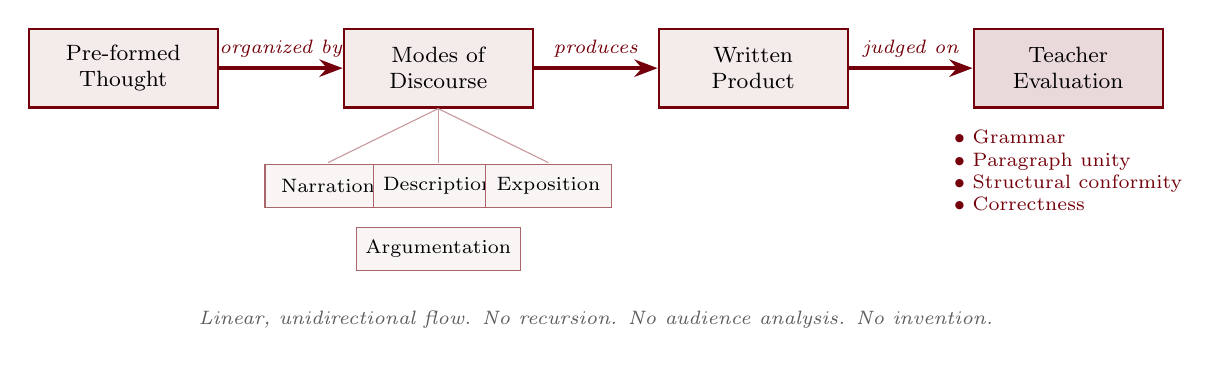
\begin{tikzpicture}[
    every node/.style={font=\footnotesize},
    box/.style={rectangle, draw=garnet, thick, fill=garnet!8,
        minimum width=2.4cm, minimum height=1cm, align=center, font=\footnotesize},
    modebox/.style={rectangle, draw=garnet!60, fill=garnet!4, minimum width=1.6cm,
        minimum height=0.55cm, align=center, font=\scriptsize},
]
% Main flow
\node[box] (thought) at (0,0) {Pre-formed\\Thought};
\node[box] (modes) at (4,0) {Modes of\\Discourse};
\node[box] (product) at (8,0) {Written\\Product};
\node[box, fill=garnet!15] (eval) at (12,0) {Teacher\\Evaluation};

\draw[-{Stealth}, very thick, garnet] (thought) -- (modes)
    node[midway, above, font=\scriptsize\itshape] {organized by};
\draw[-{Stealth}, very thick, garnet] (modes) -- (product)
    node[midway, above, font=\scriptsize\itshape] {produces};
\draw[-{Stealth}, very thick, garnet] (product) -- (eval)
    node[midway, above, font=\scriptsize\itshape] {judged on};

% Modes breakdown
\node[modebox] at (2.6,-1.5) {Narration};
\node[modebox] at (4,-1.5) {Description};
\node[modebox] at (5.4,-1.5) {Exposition};
\node[modebox] at (4,-2.3) {Argumentation};
\draw[thin, garnet!40] (modes.south) -- (2.6,-1.2);
\draw[thin, garnet!40] (modes.south) -- (4,-1.2);
\draw[thin, garnet!40] (modes.south) -- (5.4,-1.2);

% Evaluation criteria
\node[font=\scriptsize, text=garnet, align=left] at (12,-1.3) {
    $\bullet$ Grammar\\
    $\bullet$ Paragraph unity\\
    $\bullet$ Structural conformity\\
    $\bullet$ Correctness};

% Key annotation
\node[font=\scriptsize\itshape, text=black70, align=center] at (6, -3.2)
    {Linear, unidirectional flow. No recursion. No audience analysis. No invention.};
\end{tikzpicture}
\end{document}
